\documentclass{sigchi}
\pagenumbering{arabic}
\usepackage{balance}  
\usepackage{graphics}
\usepackage{times}
\usepackage{mathtools}
\usepackage{amssymb}
\usepackage{url}
\usepackage{wrapfig}
\usepackage{lipsum}


\makeatletter
\def\url@leostyle{%
  \@ifundefined{selectfont}{\def\UrlFont{\sf}}{\def\UrlFont{\small\bf\ttfamily}}}
\makeatother
\urlstyle{leo}

% Page size.
\def\pprw{8.5in}
\def\pprh{11in}
\special{papersize=\pprw,\pprh}
\setlength{\paperwidth}{\pprw}
\setlength{\paperheight}{\pprh}
\setlength{\pdfpagewidth}{\pprw}
\setlength{\pdfpageheight}{\pprh}

% set up tight list spacing
\usepackage{enumitem} 
\setlist{nolistsep,nosep}

% for toggles
\usepackage{etoolbox}


% CHANGE FROM TOGGLE TRUE TO TOGGLE FALSE FOR NON-ANONYMOUS RENDERING
% http://tex.stackexchange.com/questions/5894/latex-conditional-expression
\newtoggle{anonymous}
\toggletrue{anonymous}
 % \togglefalse{anonymous}

% CHANGE FROM TOGGLE TRUE TO TOGGLE FALSE TO HIDE COMMENTS
\newtoggle{comments}
%\toggletrue{comments}
\togglefalse{comments}

% Comment region command (from Wesley Willett)
\usepackage[usenames]{color}
\usepackage[usenames,dvipsnames]{xcolor}
\iftoggle{comments} {
  %if we want to show comments
  \newcommand {\tim}[1]{{\color{magenta}\bf{TC: #1}\normalfont}}
  \newcommand {\cesar}[1]{{\color{NavyBlue}\bf{CT: #1}\normalfont}}
  \newcommand {\ep}[1]{{\color{violet}\bf{EP: #1}\normalfont}}
  \newcommand {\bjoern}[1]{{\color{Orange}\bf{BH: #1}\normalfont}}
  \newcommand {\jasper}[1]{{\color{Blue}\bf{JO: #1}\normalfont}}
  \newcommand {\reviewer}[1]{{\color{Red}\bf{REVIEWER: #1}\normalfont}}
  \newcommand {\neil}[1]{{\color{Green}\bf{NK: #1}\normalfont}}
}{
  %if we don't want to show comments
  \newcommand {\tim}[1]{}
  \newcommand {\reviewer}[1]{}
  \newcommand {\ep}[1]{}
  \newcommand {\bjoern}[1]{}
  \newcommand {\jasper}[1]{}
  \newcommand {\cesar}[1]{}
  \newcommand {\neil}[1]{}
}


\renewcommand{\labelitemi}{{\tiny$\bullet$}}

\usepackage[pdftex]{hyperref}
\hypersetup{
pdftitle={SIGCHI Conference Proceedings Format},
pdfauthor={LaTeX},
pdfkeywords={SIGCHI, proceedings, archival format},
bookmarksnumbered,
pdfstartview={FitH},
colorlinks,
citecolor=black,
filecolor=black,
linkcolor=black,
urlcolor=black,
breaklinks=true,
}
\toappear{CS294 Report - IoET 2015 - David Culler.}

\newcommand\tabhead[1]{\small\textbf{#1}}
\newcommand\group[1]{\textit{#1}}
\newcommand\quoted[1]{\textsl{#1}}
\newcommand\name{SmartStoryboard}
\newcommand\namesp{SmartStorybaord }


\newcommand*{\layer}[1]{{\textbf{\small{\fontfamily{cmss}\selectfont{#1}}}}}

% End of preamble.

\begin{document}

\title{\name}

\iftoggle{anonymous}{
  %if anonymous
  \numberofauthors{1}
  \author{
  \alignauthor Anonymous for Submission\\
    \affaddr{...}\\
    \affaddr{...}\\
    \email{...}\\
  }
}{
\numberofauthors{1}
  \author{
  \alignauthor {Cesar Torres\quad}\\
    \affaddr{University of California, Berkeley}\\
    \email{cearto@berkeley.edu}\\
  }
}

% Some fancy Latex (that I copied) to make a title page banner
% \makeatletter
% \let\@oldmaketitle\@maketitle% Store \@maketitle
% \renewcommand{\@maketitle}{\@oldmaketitle% Update \@maketitle to insert...
%   \includegraphics[keepaspectratio, width=\linewidth]
%     {figures/teaser-sketch-2.pdf}\bigskip}% ... an image
% \makeatother


% \teaser {
%   \vspace{-8pt}
%   \centering
%     \includegraphics[width=\linewidth]{figures/teaser-sketch-2.pdf}
%     \caption{Example objects created with \name. \textit{External} and \textit{Internal} tools easily add tactility, interactivity, flexibility, and weight to objects.}
% \label{fig:teaser}
% \vspace{-8pt}
% }
 
\maketitle

\begin{abstract}
  An augmented environment coordinator for storytelling. Polls devices in a room for storytelling capabilities (e.g. light, sound, smell) and contributes a content creation tool that synthesizes output into a unique storytelling experience. 
\end{abstract}


\keywords{
  internet of things, storytelling
}

\category{H.5.m.}{Information Interfaces and Presentation (e.g. HCI)}{Miscellaneous}
% \category{D.2.2}{Design Tools and Techniques}{User interfaces (H.5.2, H.1.2, I.3.6)}



%%%%%%%%%%%%%%%%%%%%%%%%%%%%%%%%%%%%%%%%%%
%%%%%%%%%%%%%%%% INTRODUCTION %%%%%%%%%%%%
%%%%%%%%%%%%%%%%%%%%%%%%%%%%%%%%%%%%%%%%%%

\section{INTRODUCTION}
\lipsum[2]
   
%%%%%%%%%%%%%%%%%%%%%%%%%%%%%%%%%%%%%%%%%%
%%%%%%%%%%%%%%%% BACKGROUND %%%%%%%%%%%%%%
%%%%%%%%%%%%%%%%%%%%%%%%%%%%%%%%%%%%%%%%%%

\section{BACKGROUND}
Augmented reality storybook \cite{scherrer_haunted_2008}. 
Patent on modal interaction in book (i.e. greeting card sounds) \cite{iggulden_printed_1999}. 
Detecting page flips, ubicomp \cite{fujinami_page-flipping_2009}.
Telepresent story telling \cite{raffle_family_2010}. 

%%%%%%%%%%%%%%%%%%%%%%%%%%%%%%%%%%%%%%%%%%
%%%%%%%%%%%%%%%% DESIGN  %%%%%%%%%%%%%%%%%
%%%%%%%%%%%%%%%%%%%%%%%%%%%%%%%%%%%%%%%%%%

\section{SYSTEM DESIGN}
  \begin{figure}[t!]
      % \vspace{-8pt}
      \centering
      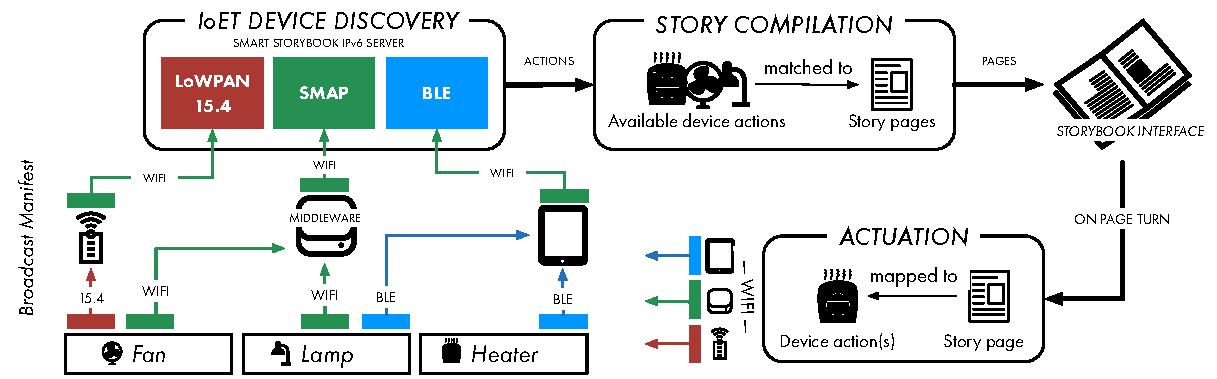
\includegraphics[keepaspectratio, width=0.5\textwidth]{figures/architecture.pdf} 
      \caption{\namesp architecture. }
      \vspace{-4pt}
      \label{fig:architecture} 
    \end{figure}

\lipsum[3]

%%%%%%%%%%%%%%%%%%%%%%%%%%%%%%%%%%%%%%%%%%
%%%%%%%%%%%%%%%% EVALUATION %%%%%%%%%%%%%%
%%%%%%%%%%%%%%%%%%%%%%%%%%%%%%%%%%%%%%%%%%

\section{BACKGROUND}
\lipsum[3]


%%%%%%%%%%%%%%%%%%%%%%%%%%%%%%%%%%%%%%%%%%%%%%%
%%%%%%%%%%%%%%%   CONCLUSION    %%%%%%%%%%%%%%%
%%%%%%%%%%%%%%%%%%%%%%%%%%%%%%%%%%%%%%%%%%%%%%%

\section{CONCLUSION}
  \lipsum[1]

%%%%%%%%%%%%%%%%%%%%%%%%%%%%%%%%%%%%%%%%%%
%%%%%%%%%%%%%%%% ACK %%%%%%%%%%%%%%%%%%%%%
%%%%%%%%%%%%%%%%%%%%%%%%%%%%%%%%%%%%%%%%%%

\section{ACKNOWLEDGEMENTS}
This work was done as a CS294 class project taught by Prof. David Culler. 
Team consisted of Aparna Dhinakaran, Michael Ho, Romi Phadte. 
The iPad Storybook application was used with permission from X. 

\balance
\bibliographystyle{acm-sigchi}
\bibliography{story}
\end{document}


